% !TeX spellcheck = sk_SK

\section{Analýza problému}
V prvej kapitole si bližšie predstavíme problematiku procesov, formalizmus Petrifow s ktorým tieto procesy vieme modelovať, a priblížime si prostredie procesne orientovaných systémov a pre

\subsection{Petriho siete}
Hovorí sa, že Carl Adam Petri vymyslel koncept Petriho sietí v auguste 1939 keď mal iba 13 rokov. Vtedy ich používal ako mnemotechnickú pomôcku na memorovanie priebehu chemických reakcií. Svoju matematickú teóriu modelovania procesov v kontexte informatiky predstavil v roku 1962 vo svojej dizertačnej práci - Komunikácia s Automatmi na technickej univerzite v Darmstadte v Nemecku. Grafickú reprezentáciu so štvorcami, kruhmi a šípkami, ktorú poznáme v súčastnosti predstavil až o tri roky neskôr, čím zožal veľký úspech v informatickej komunite. \cite{petri50years} 

Od uverejnenia Petriho dizertačnej práce v roku 1962 si jeho siete našli široké uplatnenie na poli modelovania procesov, asynchrónnych a distribuovaných systémov. 

Vo svojvej grafickej reprezentácií Pertiho sieťe modelujú udalostné systémy pomocou bipartitného grafu ktorý sa skladá z miest(kruh) a prechodov (štvorec) ktoré sú pospájané orientovanými hranami(šipkami) s označením multiplicity. Rôzne stavy procesu značíme značkami alebo inak tokenmi (bodkmi v miestach). 
Miesta (S) reprezentujú podmienky ktoré musia byť splnené na to aby mohla prebegnúť nejaká akcia v procese.
Prechody (T) reprezentujú samotné akcie v procese, ktoré menia jej stav konzumovaním a produkovaním tokenov.
Hrany (A) reprezentujú tok prostriedkov v procese a v spojení s mistami a prechodmy tvoria štruktúru procesu
Každá hrana má definovanú násobnosť (W) ktorá reprezentuje počet tokenov, ktoré sa pri spustní prechodu skonzumujú, ak hrana smeruje do prechodu, alebo vyprodukujú ak hrana vychádza z vrcholu. 

\begin{figure}[!htbp]
\centering
\includegraphics[width=6cm]{img/basic_net.svg}
\caption{Úloha}
\label{task}
\end{figure}






  Ďalším výskumom sa z pôvodného konceptu ktorý bol určený na modelovanie analýzu komunikačných systémov vyvinul nástroj, ktorý sa používa naprieč mnohými oblasťami najmä na modelovanie paralelných a distribuovaných systémov.


\subsection{Rozšírené Petriho siete}
\subsubsection{Podsiete}
\subsubsection{Roly}
\subsubsection{Dáta}
\subsubsection{Akcie}

\subsection{Petriflow}

Formalizmus Petriflow je rozšírenie Petriho sietí, ktoré bolo navrhnuté na modelovanie komplexných biznis procesov. 

Formalizmus Petriflow rozširuje Petriho siete o ďalšie komponenty. Ako základ berie Petriho siete obohatené reset, inihibitor a read hrany. Aby sa dali modelovať moderné biznis procesy pridáva Petriflow do tohto modelu roly, dátové polia a akcie.

Roly definujú kto je oprávnený spúšťať rôzne prechody.

Dátové polia definujú štruktúru dát ktoré každá inštancia procesu obsahuje počas svojho behu.

Akcie definujú vzťahy a interakcie medzi jednotlivými dátovými poľami a prechodmi.

V klasických Petriho sieťach je spustenie prechodu vždy atomická operácia. Petriflow obsahuje dva typy prechodov. Udalostné prechody, ktoré sú rovnako  ako v klasických PN sieťach atomické, avšak vždy ich spúšťa nejaká osoba(používateľ) v systéme. Druhý typ prechodu je úloha. Úlohu môžeme vnímať ako podsieť na obrázku \ref{task}. Na začiatku je úloha nepridelená, ako prvý krok je potrebné ju niekomu (aj sebe) prideliť. Následne môže toto pridelenie zrušiť, prideliť inej osobe, alebo úlohu dokončiť. My sa ďalej budeme zaoberať len úlohami.

Keďže každá úloha je samostatná sieť so štyrmi prechodmi, musíme pre každú úlohu zadefinovať roly pre všetky štyri operácie úlohy.

\begin{figure}[!htbp]
\centering
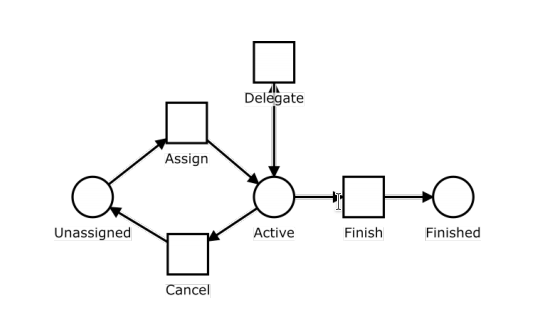
\includegraphics[width=6cm]{img/task_transition.png}
\caption{Úloha}
\label{task}
\end{figure}

\subsection{Aplikačné rozhranie}

Majme procesne orientovaný systém ktorý implementuje procesy, popísane v Petriflow. S takýmto systémom používatelia interagujú iba presne popísaným spôsobom a to spúšťaním prechodov ktoré majú podľa svojich rolí oprávnenie spúšťať (delegovať, dokončiť,... ). Pri dokončení úlohy (prechodu) musí používateľ poskytnúť dáta popísané v dátových poliach.

Keďže formalizmus Petriflow je schopný takýmto spôsobom popísať všetky interakcie používateľa so systémom je možné na jeho základe vygenerovať aj aplikačné rozhranie. Toto rozhranie sprístupní systém mimo jeho domény, zaručí autorizáciu podľa rolí, poskytne dokumentáciu o svojej štruktúre(a tým pádom aj štruktúre procesu) a zabezpečí validáciu dát, ktoré do systému používateľ odošle.

Ak by rozhranie držalo informáciu o značkovaní, a teda spustiteľnosti prechodov, mohol by nasať stav kedy aplikačné rozhranie je v stave, ktorý naznačuje, že prechod sa nedá spustiť no procesný server už je v stave, kedy je prechod spustiteľný. Keďže proces môže mať viacero spustených inštancií musia v našom systéme tieto inštancie byť adresovateľné, keďže je však predpoklad, že inštancia môže v reálnom stave vzniknúť alebo zaniknúť nemôže náš systém z rovnakých dôvodov ako pri značkovaní držať informáciu o tom, či konkrétna inštancia procesu existuje. 

Kvôli udržaniu konzistencie dát a vyhnutiu sa problémom s race conditions teda nemôže aplikačné rozhranie držať informáciu o značkovaní a teda ani spustiteľnosti prechodu na žiadnej inštancií procesu, ani o existencií inštancií procesov.

Aktuálna verzia Petriflow poskytuje relatívne granulárne informácie o autorizácií na vykonávanie akcií pomocou rolí, neobsahuje však zoznam používateľov, ich prístupových údajov a ich rolí. Na implementáciu funkčného aplikačného rozhrania, ktoré má zabezpečiť autorizáciu bude nutné dodať tieto informácie iným spôsobom.

%TODO obrazok viacero PN -> viac endpointov API - point very cloudy

\section{Špecifikácia}

V tejto kapitole najprv stručne opíšeme hlavnú funkcionalitu navrhovanej aplikácie, potom zadefinujeme funkcionálne a nefunkcionálne požiadavky na aplikáciu.

Softvér, ktorý sme sa rozhodli implementovať bude slúžiť ako rozhranie medzi procesným serverom a internetom. Bude umožňovať klientovi pripojiť sa na procesný server cez internet, autentifikovať sa, získať informácie o dátach v prechodoch petriho siete a bude umožňovať modifikovať stav siete (procesu) spúšťaním prechodov.

\subsection{Funkcionálne požiadavky}

\begin{enumerate}
\item Rozhranie bude umožňovať administrátorovi registrovať používateľov a priraďovať im roly
\item Umožní administrátorovi za behu pridať nové koncové body a meniť, alebo vymazať aktuálne nasadené koncové body
\item Umožní prihlásenie používateľa pomocou štandardného autentifikačného protokolu.
\item Autentifikovaným používateľom umožní prístup k dátam z tých prechodov ktoré majú právo čítať podľa ich roly.
\item Autentifikovaným používateľom umožní spúšťať prechody ktoré majú právo spúšťať podľa ich roly.
\item Pri spúšťaní prechodu prebehne validácia vstupných dát. V prípade nevalidných alebo nekompletných dát nepovolí spustenie prechodu.
\item Rozhranie poskytne online dokumentáciu prechodov v sieti, táto dokumentácia bude zahŕňať URL prechodu, potrebné dátové polia na spustenie prechodu a roly, ktoré sú oprávnené prechody spúšťať.
\item Rozhranie poskytne aplikačné rozhranie viacerým sieťam s rôznou štruktúrou. A viacerým inštanciám týchto sietí.
\end{enumerate}

\subsection{Nefunkcionálne požiadavky}
\begin{enumerate}
\item Rozhranie bude škálovateľné
\item Rozhranie bude zabezpečené štandardnými bezpečnostnými prvkami
\item Rozhranie bude bežať na serveri poskytnutom Fakultou Elektrotechniky a Informatiky na Slovenskej Technickej Univerzite v Bratislave.
\end{enumerate}

\section{Návrh}
V tejto kapitole preberieme proces návrhu nášho aplikačného rozhrania. V časti Prípady použitia si opíšeme interakcie rôznych používateľov s naším systémom a očakávanú odpoveď nášho systému na tieto interakcie.

Následne v časti Štruktúra aplikačného rozhrania opíšeme ako navrhujeme štruktúru aplikačného rozhrania tak aby dokázala pokryť všetky interakcie, ktoré vyplývajú z definície v Petriflow. 

V časti Architektúra systému priblížime ako navrhujeme systém tak, aby spĺňal požiadavky na škálovateľnosť bezpečnosť a funkcionalitu.

Napokon v časti Operácia systému predstavíme control flow navrhnutej aplikácie.


\subsection{Prípady použitia} \label{usecases}
V kapitole Špecifikácia v časti Funkcionálne požiadavky ja uvedené aké interakcie očakávame, že používateľ a administrátor musia byť schopný vykonávať s naším systémom. Následné interakcie a ďalej analyzujeme v tejto časti našej práce. 

\subsubsection{Registrácia modelu}
Prvý prípad použitia je registrácia modelu. Aktér ktorý môže registrovať modely je len administrátor. Pri tejto akcií administrátor poskytne nášmu systému informácie o štruktúre procesu vo formáte petriflow, zoznam používateľov im prislúchajúcich rolí v \acrshort{xml} a unikátny identifikátor siete.

Pokiaľ chce administrátor upraviť nasadený proces spustí proces registrácie nanovo s upravenými údajmi o sieti, používateľoch a rolách.

Administrátor taktiež môže sieť vymazať.

\subsubsection{Získanie informácie o prechode}
Keď už sú sieť aj používatelia úspešne zaregistrovaný, si môžu používatelia, vyžiadať informácie o prechode. Tieto informácie budú poskytnuté len používateľovi s rolou oprávnenou na čítanie dát z daného prechodu.

\subsubsection{Vykonanie akcie na prechode}
Používatelia s príslušnými rolami môžu taktiež vykonávať akcie na prechodoch. Tieto akcie vyplývajú z definície petriflow a patrí medzi ne assign, delegate, cancel, a finish. Na každú z týchto akcií potrebuje používateľ mať opávnenie (rolu, ktorá je oprávnená vykonávať túto akciu), a každá z nich vyžaduje iné vstupné dáta.

\subsubsection{Autentifikácia}
Z požiadavky na bezpečnosť aplikácie vyplýva ešte prípad použitia, kedy sa používateľ autentifikuje, aby nadobudol identitu rozpoznanú našim systémom a boli mu pridelené roly.

\subsection{Štruktúra aplikačného rozhrania}
Pri návrhu štruktúry aplikačného rozhrania treba dbať hlavne na prehľadnosť a jednoznačnosť rozhrania. Naše aplikačné rozhranie musí jednoznačne pokryť všetky možné koncové body, ktoré sú možné vygenerovať z procesného modelu Petriflow. Zároveň sme sa rozhodli pri návrhu rozhrania čo najviac držať návrhového vzoru \acrshort{rest}. 

Vzor \acrshort{rest} je už mnoho rokov štandardom pri návrhu aplikačných rozhraní na internete. Jeho základný princíp je že medzi serverom a klientom sa bude presúvať textová reprezentácia objektov, tieto objekty sú adresované pomocou parametrov v URL danom volaní REST koncového bodu. Na manipuláciu s objektami na konkrétnych URL sa vužívajú HTTP medóty GET, POST, PUT, PATCH, DELETE, atď.  sa využívajú . GET získava objekt, POST vytvára nový, DELETE objekt vymazáva, atď.

Objekty, pre ktoré musí náš systém vyprezentovať aplikačné rozhranie sú  procesy (Petriho siete), inštancie týchto procesov a prechody na týchto inštanciách. Ak by sme mali implementovať plné RESTful \acrshort{api} so štandatrnou štrukúrou URL by mala nasledovný formát.

\[/net/[netID]/instance/[instanceID]/transition/[transitionID]/[operation] \]

Keďže však naše rozhranie bude poskytovať len možnosť spúšťať operácie na konkrétnych prechodoch a hierarchia objektov bude vždy rovnaká, rozhodli sme sa skrátiť tento zápis a vynechať typy objektov z URL na nasledovný.
\[/[netID]/[instanceID]/[transitionID]/[operation] \]
Okrem automaticky generovaný ch ciest potrebujeme ešte zadefinovať cesty ktoré bude používať administrátor systému na obslužné dotazy, pomocou ktorých bude administrátor schopný pridávať odoberať a získavať informácie o modeloch. Pre tieto operácie vyhradíme adresu "/".

Na ukážke \ref{alg:urls_example} môžeme vidieť  Príklad URL Pre verejné a pre obslužné administrátorské \acrshort{api}.

\begin{table}[caption={Ukážka URL ciest k úlohe},label={alg:urls_example}]
\begin{tabular}{lllll}
Používateľské API     & URL                       & Metóda       &                                      &  \\
                      & /ExampleNet/0/t1          & {[}GET{]}    & Získanie dátových polí               &  \\
                      & /ExampleNet/0/t1/assign   & {[}POST{]}   & Priradenie úlohy sebe                &  \\
                      & /ExampleNet/0/t1/delegate & {[}POST{]}   & Priradenie úlohy inému požívatľovi   &  \\
                      & /ExampleNet/0/t1/cancel   & {[}POST{]}   & Zrušenie priradenia                  &  \\
                      & /ExampleNet/0/t1/finish   & {[}POST{]}   & Dokončenie úlohy                     &  \\
Admininstrátorské API & /                         & {[}POST{]}   & Registrácia nového modelu            &  \\
                      & /                         & {[}GET{]}    & Vypísanie zoznamu nasadených modelov &  \\
                      & /                         & {[}DELETE{]} & Vymazanie modelu                     & 
\end{tabular}
\end{table} ction{Architektúra systému}
Aby sme splnili požiadavku na jednoduché škálovanie aplikácie a pre sprehľa    dnenie archite    ktúry zvolili sme si architektúru mikroservisov. Táto architektúra pozostáva z viacerých oddelených častí (servisov), každá z týchto častí má svoju jasne definovanú funkciu. Takéto mikroservisy sú jednoducho testovateľné, dajú sa nasadzovať postupne a nezávisle od seba a softvér navrhnutý v tejto architektúre býva spravidla robustný a vysoko škálovateľný.

Jedna z požiadaviek na náš systém je aby bolo aplikačné rozhraní možné meniť za behu systému. Pri návrhu sme zvažovali dva spôsoby ako zabezpečiť tuto funkcionalitu.

Jeden spôsob by bol napísať univerzálny kód koncového bodu, ktorý by príjmal akékoľvek požiadavky a potom pomocou internej logiky rozhodol, či je dotaz korektný a vykonal by adekvátnu akciu.  Takýto koncový bod by bol schopný okamžite zmeniť svoje nastavenie pri zmene procesného modelu. Nevýhodou tohto riešenia je že koncový bod by musel obsahovať logiku ktorá by držala štruktúru modelu a vedela by na jej základe spracovávať dopyty. Ďalšia nevýhoda tohto prístupu spočíva v nutnosti pregenerovať online dokumentáciu pri každej zmene modelu. Po hlbšej analýze dostupných technológií sme zistili, že zmena dokumentácie za behu servera nieje štandardná operácia ktorá je podporovaná v serverových frameworkoch. 

Druhý spôsob by bol mať jednu službu, ktorá je schopná čítať procesné modely v Petriflow a na ich základe je schopná vygenerovať kód, mikroslužby, ktorá je schopná obslúžiť iba konkrétny model (množinu modelov).  Vygenerovanú službu následne spustí.
Výhodou tohto prístupu je že keďže vygenerovaný kód nemusí obsahovať logiku, ktorá rozhoduje o tom, či je volanie validné a na ktorý koncový bod smeruje, tento kód je už dopredu vygenerovaný generátorom. Toto znižuje komplexitu kódu koncových bodov a zvyšuje ich priepustnosť. Ďalšou výhodou je že tento prístup nám umožňuje využívať štandardný spôsob generovania dokumentácie keďže ju nemusíme meniť za behu. Nevýhodou tohto prístupu je, že pri zmene procesného modelu môžeme očakávať nejaký čas, kedy bude rozhranie nedostupné. Keďže však pracujeme s predpokladom, že procesné modely sa nebudú meniť až tak často napriek tejto nevýhode sme sa rozhodli postupovať pri návrhu ďalej s týmto modelom. 

Na diagrame \ref{architecture} vidíme návrh architektúry systému.Softvér sa bude skladať z troch hlavných služieb: generator service, relay service a auth service. 
\begin{figure}[!htbp]
	\centering
	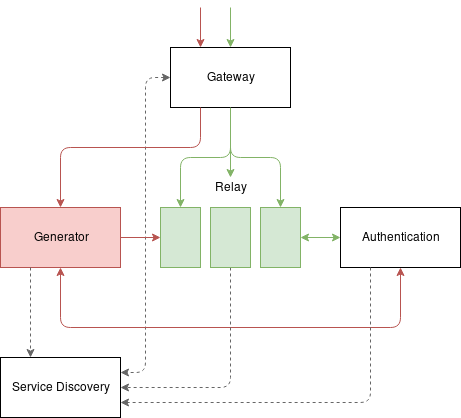
\includegraphics[width=10cm]{img/architecture.png}
	\caption{Architektúra rozhrania}
	\label{architecture}
\end{figure}

\begin{itemize}
\item Generator je služba, ktorá bude registrovať a zostavovať koncové body. Je to služba, na ktorú sa pripojí administrátor, zadá štruktúru siete a zoznam používateľov a rolí. Táto služba následne zaregistruje používateľov a ich roly, vygeneruje kód pre službu relay a túto službu spustí.
\item Relay je služba, ktorá obsahuje vygenerovaný kód koncových bodov. Táto služba bude poskytovať dokumentáciu dostupných koncových bodov. bude poskytovať samotné koncové body a pri zavolaní koncového bodu sa bude starať o validáciu prijatých dát.
\item Autentifikačná služba sa stará o autentifikáciu používateľov a prideľovanie rolí používateľom
\item Gateway služba poskytuje rozhranie medzi internetom a našou doménou. Vonkajšiemu svetu prezentuje len služby ktoré majú byť dostupné z internetu. Zároveň poskytuje funkcionalitu load balancera.
\item Service discovery je služba ktorá monitoruje stav všetkých ostatných kontajnerov a vie poskytnúť informácie o stave systému, toto je potrebné na správnu operáciu load balancera.
\end{itemize}


\subsection{Operácia systému}
V tejto časti si priblížime akým spôsobom navrhujeme flow jendotlivých procesov v našom systéme. Najprv popíšeme proces autentifikácie a zavolania koncového bodu klientom a potom popíšeme volanie obslužného koncového bodu administrátorom
\subsubsection{Používateľské API}
Na diagrame \ref{api_operation} vidíme vo vrchnej časti proces prihasenia používateľa a v dolnej časti vykonanie dopytu na procesný server.


\begin{figure}[!htbp]
	\centering
	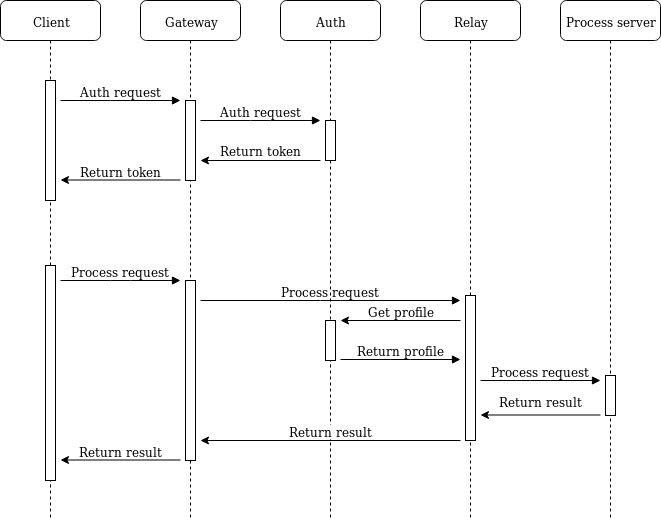
\includegraphics[width=10cm]{img/api_operation.png}
	\caption{Operácia rozhrania}
	\label{api_operation}
\end{figure}

Počas procesu prihlásenia používateľ najprv odošle dopyt na prihlásenie našemu \acrshort{api}.  Gateway ho presmeruje na autorizačný servis, ten overí jeho prihlasovacie údaje, ak sú správne vráti klientovi autorizačný token. Autentifikácia v takejto forme prebieha len pred prvým dopytom. K ďalším dopytom už klient priloží tento autorizačný token. 

Proces dopytu na procesný server je zložitejší. Najprv klient pošle dopyt na náš systém, Gateway ho nasmeruje na relay servis. Ak klient odoslal dopyt na korektnú adresu Relay servis musí potvrdiť identitu klienta. Identitu klienta overuje pomocou priloženého autorizačného tokenu ktorý klient musí poskytnuť. Relay servis zistí identitu klienta tak, že pošle interný dopyt na  auth servis a podľa tokenu si vypýta profil používateľa s jeho rolami.  Pokiaľ má klient rolu potrebnú na spustenie konkrétnej akcie na prechode, ak je to potrebné Relay servis vykoná validáciu dát  v dotaze odošle dopyt na procesný server.  Odpoveď z procesného servera sa následne propaguje spať cez gateway servis ku klientovi.
 
Keďže nebudeme mať prístup k nasadenému procesnému servisu bude volanie tohto serveru vykonané iba ako volanie prázdnej funkcie. Od tejto funkcie očakávame, že v prípade, ak prebehla akcia na prechode v poriadku vráti buď príslušné dáta alebo prázdnu odpoveď.  Ak sa klient pokúsi spustiť prechod, ktorý v konkrétnej inštancií procesu nieje spustiteľný alebo ak daná inštancia procesu neexistuje, očakávame, že volanie vráti príslušnú chybu. 

\subsubsection{Obslužné API}
Proces autentifikácie pri obslužnom volaní bude prebiehať rovnakým spôsobom ako pri  používateľskom volaní. Administrátor dostane autentifikačný token, pomocou ktorého pri všetkých ďalších volaniach preukazuje svoju identitu.

Administrátor zadá požiadavku na zmenu rozhrania, bude presmerovaný na generator service. Ten rozanalyzuje nový procesný model, následne a odošle dopyt na auth service na registráciu nových používateľov. Paralelne vygeneruje nový kód pre relay service a spúšťa jeho kompiláciu a tetovanie. Po úspešnom ukončení oboch procesov odošle dopyt na vypnutie starého relay servisu a spúšťa novú verziu.

Na diagrame \ref{change_operation} môžeme vidieť tento proces zmeny aplikačného rozhrania.

\begin{figure}[!htbp]
	\centering
	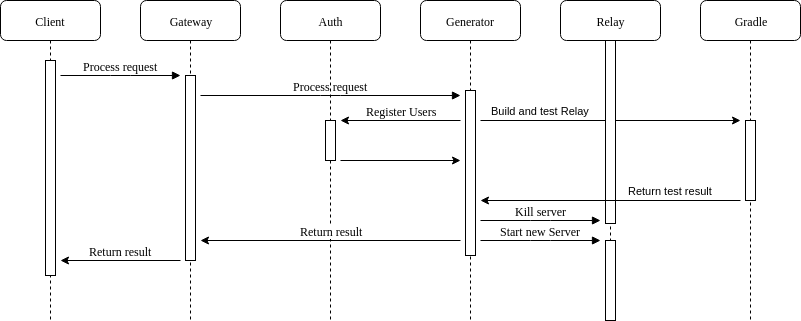
\includegraphics[width=10cm]{img/api_operation_change.png}
	\caption{Proces zmeny rozhrania}
	\label{change_operation}
\end{figure}


\section{Implementácia}
V tejto kapitole najprv predstavíme technológie ktoré sme použili pri implementácií nášho systému, Následne predstavíme štruktúru implementovaného projektu a opíšeme ako prebiehal proces zakladania projektu a repozitárov s kódom. 
Nasledujúce časti práce venujeme implementácií jednotlivých služieb, ktoré sme implementovali ako časti nášho Cloudového riešenia.
Na záver kapitoly predstavíme  platformu na ktorú sme implementované riešenie nasadzovali a popíšeme kroky nevyhnutné na sadanie nášho systému.  

\subsection{Použité technológie}
V tejto časti predstavíme technológie ktoré sme vybrali na realizovanie implementácie nášho systému. Pri výbere technológií sme dbali najmä na ich relevanciu na poli Cloudových riešení, snažili sme sa však vybrať aj novšie, zajujímavé technológie ktoré v tomto odvetví ešte len začínajú. 

\subsubsection{Kotlin}
Kotlin je relatívne nový programovací jazyk, projekt Kotlin bol po prvý krát zverejnený v roku 2011 spoločnosťou JetBrains(Andrey Breslav). Bol vyvinutý ako moderný staticky typovaný jazyk, ktorý podporuje rýchlu kompiláciu do javy. V roku 2017 ohlásil Google podporu pre Kotlin v operačnom systéme Android. V rovnakom roku ohlásil Pivotal Software oficiálnu podporu pre Kotlin vo verzii 5.0 ich frameworku Spring.

Kotlin sa dá buď transpilovať do jazyka Java, alebo JavaScript, alebo sa dá kompilovať priamo do spustiteľného binárneho súboru pe všetky bežné operačné systémy (Linux, Windows, Android, iOS).

Jazyk bol navrhnutý tak, aby bol čo najviac čitateľný, čo najviac sa vyhol potrebe písať zbytočný, alebo duplicitný kód a aby sa čo najviac vyhol chybám pri behu systému, a odchytal chyby už pri kompilácií. Na nasledujúcich príkladoch si ukážeme akými spôsobmi dosiahli tvorcovia tohto jazyku tieto ciele. 

V jazyku Kotlin sa deklarujú premenné pomocou kľúčových slov val alebo var, takto deklarujeme buď konštanty, alebo premenné. samotný typ premennej je vo väčšine prípadov odvodený z hodnoty ktorú premennej pridelíme. V prípade, že zadefinujeme premennú pomocou var a nemutujeme jej obsah, kompilátor hlási varovanie, že premenná môže byť zmenená na konštantu. Tento prístup však funguje len pri primitívnych dátových typoch. Pri kontajneroch sa uplatňuje rovnaký princíp použitím imutabilných dátových štruktúr list, map, a ďalšie. Ak chceme zadeklarovať list ktorého obsah plánujeme meniť musíme použiť typ mutableList. 

Ďalšie vylepšenie typového systému prichádza implementáciou nulovateľných typov. Tento princíp obmedzuje potrebu používania try catch blokov a na miesto toho ich nahradzuje nulovateľnými typmi. Ak pracujeme s funkciou, ktorá nemusí vždy vrátiť dáta, jej vstupný typ bude nulovateľný. Pri práci s takýmito nulovateľnými typmi nám kompilátor núti ošetriť prípady, kedy premenná obsahuje null. Na ukážke kódu \ref{alg:kt_null} vidíme, príklad funkcie, ktorá vracia nulovateľný String?. Ak sa pokúsime pristúpiť k parametru length tejto premennej pred tým ako ošetríme nulový prípad, kompilátor vyhlási kompilačnú chybu a nedovolí nám kód skompilovať. Ak by sme tento prípad neošetrili v Jave by došlo k chybe až pri behu programu. 

Ak korektne ošetríme nulový prípad kompilátor zmení ty premenenej na nenulovateľný a dovolí nám ďalej pracovať s premennou, lebo už je zaučené, že nenastane chyba pri prístupe k dátam. 


\begin{lstlisting}[ caption={Ukážka funkcie typov v jazyku Kotlin},label={alg:kt_null},language=Kotlin]
// vráti null alebo String
fun maybeGetString():String?

// typ String? - môže obsahovať null, nieje nutné typ explicitne definovať je inferovaný z výstupného typu finkcie
val variable = maybeGetString()

// nastane chyba pri kompilácií, lebo nieje ošetrený prípad, kedy je valiable null
print(variable.length)

if(isNullOrEmpty(variable){
	variable = "placeholder"
}

// nenastane chyba pri kompilácií, lebo bol ošetrný nulový priípad
// typ String - už nemôže byť null, iba string
print(variable.length)
\end{lstlisting}


Ďalšie zlepšenie jazyka ktoré je veľmi užitočné pri práci s frameworkom Spring sú dátové triedy. Ak by sme v Jave chceli vytvoriť jednoduchú triedu, ktorá len drží dáta, musíme zadeklarovať triedu, jej konštruktor, dátové polia, a funkcie na nastavovanie a čítanie polí. v jazyku Kolin vieme zadeklarovať dátovú triedu pomocou jednoriadkového príkazu. Na ukážke kódu \ref{alg:kt_dataclass} vidíme príklad dátovej triedy Person s povinnými prvými dvomi poľami firstName a lastName a nepovinnými poľami age a height. Pole firstName je konštantné, preto sa nebude dať meniť nie je nutné vynechať implementáciu nastavovacej funkcie ako v Jave. Polia age a height sú nepovinné.  
 
V jazyku Kotlin je implementovaný aj princíp pomenovaných argumentov. To znamená, že konštruktor našej dátovej triedy Person môžeme zavolať s ľubovoľnou kombináciou nepovinných argumentov. 

\begin{lstlisting}[ caption={Ukážka dátových tried a pomenovaných argumentov v jazyku Kotlin},label={alg:kt_dataclass},language=Kotlin]
	data class Person(
		val firstName: String,
		var lastName: String,
		var age?: Int,
		var height:? Int)

  val p1 = Person("Jozef", "Mrkva", height=180)		
	\end{lstlisting}



My sme zvolili jazyk Kotlin pre náš projekt hlavne kvôli vylepšeniam v systéme typovania a zmenšenému boilerplatu. Ďalej nám využitie tohto jazyka umožnila bezproblémová integrácia s frameworkom Stping a ostatnými knižnicami v jazyku Java.	

\subsubsection{IntelliJ IDEA}


\subsubsection{Gradle}
Gradle je voľne šíriteľný nástroj na automatizáciu zostavovania softvéru. Je stavaný na to aby bol schopný zostaviť takmer ľubovoľný program.  V našom projekte Gradle použijeme na manažment závislostí, kompiláciu kódu a spustenie samotného skompilovaného programu. 

Gradle urýchľuje proces zostavovania aplikácií použitím pokročilej techniku memoizácie pri každom kroku zostavovania. Pri zostavovaní teda spúšťa len procesy ktorým sa zmenili vstupné dáta  a teda očakávame iný výstup. Pri nezmenených dátach nieje nutné bežať tieto procesy znova. Gradle dokonca umožňuje vybudovanie vyrovnávacej pamäte ktorá je následne zdieľaná medzi viacerými zariadeniami.

Gradle beží v JVM a na jeho spustenie postrebujeme mať k nainštalovaný Java Development Kit. Gradle však nieje obmedzený iba na zostaveovanie Java apliácií, medzi jayky ktoré je schopný zostavovať patri aj C++, Python, a mnoho ďalších.

Konfigurácia nástroja Gradle prebieha pomocou konfiguračného súboru napísaného v jazyku Groovy. Keďže Gradle pomocou pluginov vždy implementuje všetky konenčné nastavnia a je nutné nastaviť iba veci, ktoré niesú podľa bežných konvencí, tieto konfiguračné  súbory sa v našom prípade ukázali ako veľmi krátke a prehľadné. 

\subsubsection{Spring framework}
Spring framework je open source projekt, udržiavaný  Pivotal Software, Inc. Je to Java framework a ekosystém pridružených modulov, pomocou ktorého sa dá implementovať takmer akýkoľvek biznisový zámer.  

Základom Spring frameworku je Spring IoC Container ktorý obsahuje základné prostredie Spring frameworku. Do tohto kontajnera sa následne dajú pridať ľubovoľné moduly z rozsiahleho ekosystému Spring, ktorý obsahuje Spring moduly ale aj integrácie so softvérom tretích strán.

Jadro Spring je založený na návrhovom vzore Inversion of Control, (inak aj Dependency Injection). Spring implementácia tohto modelu spočiva v použití tvz Beanov. Beany sú jednoduché singleton objekty ktoré obsahujú biznis logiku aplikácie. Pridaním anotácií týmto jednoduchým objektom im definujeme závislosti. Tieto v spolupráci s XML konfiguráciou a ak je to treba war súborom tretej strany spustia, napr. webový server, ktorý následne importuje inštancuje náš Bean a využíva z neho biznis logiku ktorú sme implementovali. 
Tento prístup sa snaží uľahčiť prácu programátorom tým, že eliminuje potrebu implementácie platformy a umožňuje im sa viac sústrediť na biznis logiku aplikácie.  

Spring framework implementuje aj vlastný systém na realizovanie aspektovo orientovaného programovania.

\subsubsection{Spring Boot}
Spring Boot je jeden z projektov ekosystému Spring, ktorý sa snaží uľahčiť zakladanie projektov a konfiguráciu Spring projektov. Tento cieľ dosahuje uplatnením uprednostňovaním konvencie pred konfiguráciou. Toznamená, že developeri Sprignu pripravili dopredu nakonfigurované projekty, ktoré riešia bežné prípady použitia Spring Frameworku. 

Medzi tieto projekty, tzv. startery patrí napr. Spring Boot Web Starter ktorý zabezpečuje funkcionalitu webového servera, Spring Boot Security Starter ktorý pridáva funkcionalitu autentifikácie a autorizácie, Spring Boot Data JPA Starter ktorý pridáva integráciu s perzistentnými úložiskami dát. Tieto startery obsahujú integráciu s vybranými nástrojmi, ktoré prednastavili developeri Springu podľa toho ako to oni považovali za najlepšie. V niektorých prípadoch obsahujú integrované servlety tretích strán, napríklad už spomínaný Web Starter obsahuje webový servlet Apache Tomcat. 

V rámci ekosystému Spring Boot existuje aj nástroj Spring Initializr \cite{initializr}, pomocou tohto nástroja je možné vygenerovať a stiahnuť archív so Spring Boot projektom. Tento nástroj nám umožňuje nastaviť niektoré parametre projektu ako verziu Spring Boot, programovací jazyk, a umožňuje nám pridať do projektu základné závislosti.   

\subsubsection{Spring cloud}
Pri implementácií cloudových aplikácií sa developeri často stretávajú s podobnými problémami ako napríklad ako distribuovať konfiguráciu v rámci aplikácie, ako riešiť smerovanie medzi viacerými kontajnermi, ako riešiť distribuované relácie používateľov. Ekosystém Spring Cloud stavia na princípoch Spring Boot, a poskytuje nástroje na rýchly vývoj stabilných a výkonných cloudových systémov. 

Spring Cloud obsahuje mnohé projekty, ktoré implementujú rôznu rozšírenú funkcionalitu, na zabezpečenie bezpečnosti, výkonu, vysokej škálovateľnsoti a spoľahlivosti.s
My z nich budeme využívať nasledovné:

\begin{itemize}
\item Spring Cloud Config - Centralizovaný systém na distribúciu externej konfigurácie v cloudovom prostredí. Umožňuje prístup ku konfigurácií uloženej v cetrálmin git repozitári priamo z prostredia Spring Frameworku.
\item Spring Cloud Netflix - Poskytuje intregáciu s Netflix OSS komponentami ako Eureka(service discovery), Hystrix(circuit breaker), Zuul(Router, load balancer), Archarius(cloud config) a ďalšími. Z tohto projektu budeme využívať iba projekt Eureka ako service discovery.
\item Spring Cloud Security - Poskytuje podporu pre OAuth2 a komplexné riešenie autentifikácie a autorízácie v distrubuovanom Cloudovom prostredí.
\item Spring Cloud Gateway - Nástroj na smerovanie a load balalncing postavený na princípoch reaktívneho programovania.
\end{itemize}




\subsubsection{Git}
Git je najpoužívanejší nástroj na kontrolu revízií na svete. Bol vytvorený Linusom Torvaldsom v roku 2005 na kontrolu revízií pri vývoji jadra Linuxu. A rovnako ako Linux bol zverejnený na voľné používanie. V našom projekte sme použili git na kontrolu revízií samotného kódu našej aplikácie. Zároveň sme využili Java knižnicu JGit \cite{jgit}. Bola vyvinula a je ďalej udržiavaná spoločnosťou Eclipse Foundation, Inc. Táto knižnica nieje len wrapper na natívneho git klienta, je to plnohodnotná implementácia Git klienta v jazyku Java, toto nám zabezpečuje plnú funkcionalitu Git klienta bez nutnosti inštalovať Git samostatne. 

\subsubsection{Insomnia}
Insomnia \cite{insomnia} je voľne šíriteľný softvér vyvíjaný spoločnosťou Floating Keyboard Software Inc. Je určený na testovanie REST a GraphQL služieb. Je to alternatíva ku známemu programu Postman. Je postavený na platforme Electron s použitím knižnice React. Insomnia nám dovolí vytvoriť a uložiť viacero testovacích dopytov, ktoré môžeme neskôr spustiť a overiť ich správne fungovanie. Insomnia taktiež podporuje autentifikačný protokol OAuth2. Okrem štandardných HTTP volaní podporuje aj čoraz viac populárny protokol GraphQL



\subsection{Štruktúra projektu}
%todo rename
Naše aplikačné rozhranie sme implementovali ako cloudové riešenie s piatimi rôznymi kontajnermi: Gateway, Generator, Auth, Service Discovery a Relay. Implementáciu jednotlivých kontajnerov opíšeme v ďalčích kapitolách.

Všetky projekty sme vytvárali pomocou Spring Inilitalizr. Na obrázku \ref{initializr} môžeme vidieť ukážku konfigurácie Spring initializr pre prvú službu Generator service.  Ako typ projektu sme zvolili Gradle, ako programovací jazyk sme zvolili Kotlin, verziu Spring Boot sme nechali predvolenú, vždy je prednastavená aktuálne najnovšia stabilná verzia, v čase, keď sme zakladali projekt to bola 2.1.1. Dalej sme zadali meno balíka nášho projektu a artefakt, ktorý sa použije aj ako názov priečinka a meno projektu. Na koniec sme pridali základné moduly, ktoré sme použili v jednotlivých projektoch.

 \begin{figure}[!htbp]
	\centering
	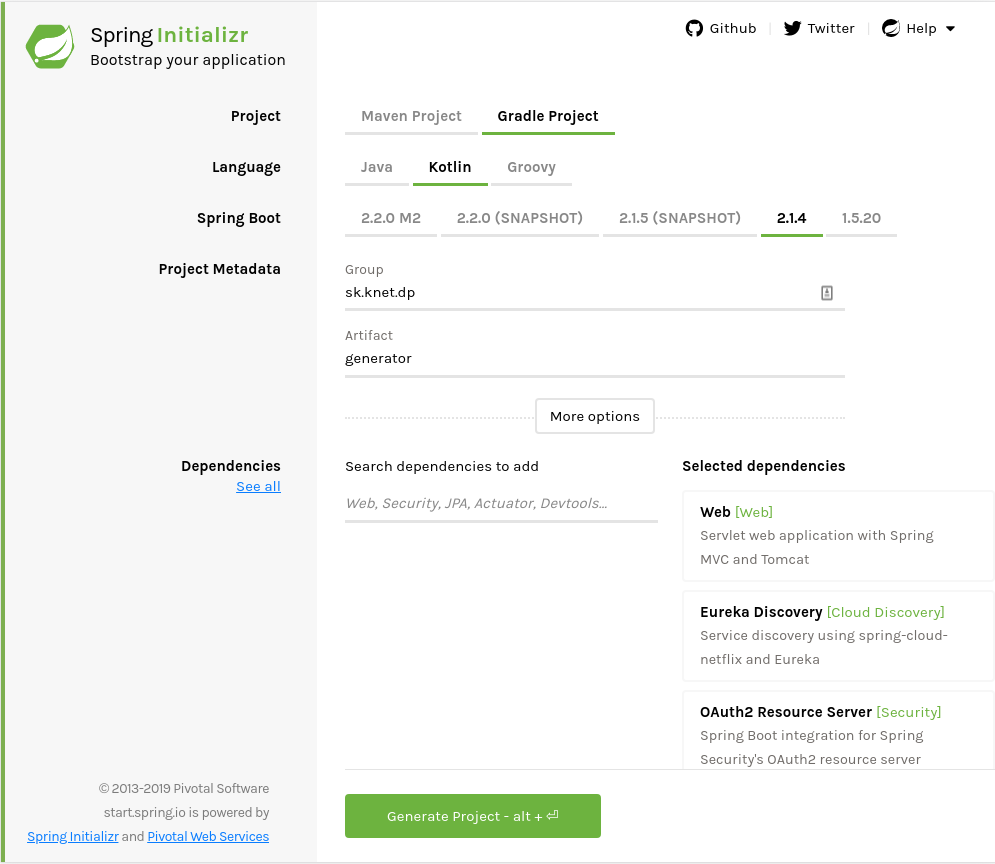
\includegraphics[width=16cm]{img/initializr.png}
	\caption{Ukážka nastavenia Spring Initializr}
	\label{initializr}
\end{figure}

Zdrojovy kód týchto kontajnerov sme rozdelili do dvoch Git repozitárov. Relay service sme pre zjednodušenie automatického nasadzovania umiestnili do vlastného repozitára\cite{dp_relay}. Ostatné služby sú uložené v spoločnom repozitári \cite{dp_repo}. 



\subsection{Generator service}
Tento servis je základný stavebný kameň nášho rozhrania, jeho úlohou je na základe vstupu v podobe procesného modelu vo formáte Petriflow vygenerovať a spustiť inštancie relay service, ktorý bude prijímať samotné požiadavky od klienta. Základná operácia vygenerovania koncového dobu má nasledovné kroky:
prijatie požiadavky,
čítanie súborov Petriflow a súborov s používateľmi,
registrácia používateľov,
príprava repozitára,
generovanie kódu
a kompilácia a spustenie relay.

\subsubsection{Prijatie požiadavky}
Pre funkciu pridania požiadavky je v našom systéme vyhradená základná URL "/[POST]", na tejto URL je funkcia, ktorá berie ako parametre súbor s procesným modelom, súbor s používateľmi a unikátny identifikátor siete. Súbor s modelom je v štandardnom formáte Petriflow. Súbor s používateľmi je vo formáte \acrshort{xml} so štruktúrou popísanou \acrshort{xsd} súborom v prílohe \ref{att:xsd}. Tento XSD súbor je poskytnutý aj v rámci dokumentácie v \acrshort{openapi}. Na príklade súboru v ukážke kódu \ref{alg:example_users} môžeme vidieť že súbor obsahuje zoznam používateľov s menom, heslom a zoznamom ich rolí.

\begin{lstlisting}[float, caption={Príklad súboru s používateľmi},label={alg:example_users},language=XML]
<?xml version="1.0" encoding="UTF-8"?>
<document xmlns:xsi="http://www.w3.org/2001/XMLSchema-instance" xsi:noNamespaceSchemaLocation="./users_schema.xsd">
	<user name="admin" password="SecureAdminPass">
		<role id="client"/>
		<role id="bureau_agent"/>
		<role id="loan_officer"/>
		<role id="underwriter"/>
		<role id="property_appraiser"/>
		<role id="account_clerk"/>
	</user>
	<user name="user1" password="SecureUser1Pass">
		<role id="bureau_agent"/>
		<role id="underwriter"/>
		<role id="account_clerk"/>
	</user>
	<user name="user2" password="SecureUser2Pass">
		<role id="client"/>
		<role id="loan_officer"/>
		<role id="property_appraiser"/>
	</user>
</document>
\end{lstlisting}

Funkciu registrácie môže spustiť iba administrátor systému(Viac v časti Auth Service \ref{section_auth}).

Tieto súbory sa uložia do priečinka na servery s názvom Net[ID siete] a Users[ID siete]. V prípade, že už existujú súbory s rovnakým ID tieto súbory sa prepíšu a tým zaručujeme funkcionalitu zmeny siete.

Ukladanie súboru s heslami v textovej forme je v produkčnej aplikácií neprípustné, preto pred uložením vytvoríme hash hesla štandardným spôsobom kompatibilným so Spring Security.

Okrem požiadavky na pridanie siete môže administrátor spustiť aj požiadavku na vymazanie siete. V takomto prípade sa vymažú súbory s ID danej siete a ďalšie kroky postupujú rovnako ako pri registrácií.

\subsubsection{Čítanie súborov Petriflow a súborov s používateľmi}
Na čítanie \acrshort{xml} súborov používame štandardnú knižnicu JAXB \cite{jaxb}. Táto knižnica podľa \acrshort{xsd} súborov vygeneruje triedy, so rovnakou štruktúrou ako majú entity v \acrshort{xml}.

Vygenerovali sme teda dva balíky, jeden balík s triedami v jazyku Java z definície Petrfilow a jeden s triedami z definície nášho súboru s používateľmi.

Následne pri čítaní súborov použijeme triedu Unmarshaller balíka JAXB, ktorý prečíta textový súbor \acrshort{xml} a vráti Java objekty s dátami zo súborov. Keďže jazyk kotlin, v ktorom pracujeme je plne kompatibilný s jazykom Java, s týmito objektami môžeme ďalej pracovať ako so štandardnými kotlin dátovými objektami.

\subsubsection{Registrácia používateľov}
Keď už máme dáta s používateľmi a modelom, zaregistrujeme používateľov do našej autentifikačnej služby.

Registrácia používateľov sa realizuje pomocou HTTP volania na Authentication service. Servisu poskytneme prihlasovacie meno a heslo používateľa. Aby sme predišli konfliktom v menách používateľov medzi jednotlivými sieťami, pred prihlasovacie mená pridáme ID siete a tým pádom sú všetci používatelia jednej siete v samostatnom menovom priestore.

\subsubsection{Príprava repozitára}
Na spustenie Spring Boot kontajnera treba okrem kódu so samotnými koncovými bodmi aj základnú konfiguráciu. Pre zjednodušenie procesu generovania kódu stiahneme predpripravenú konfiguráciu zo separátneho git repozitára \cite{dp_relay}. V tomto repozitári je predpripravený Spring Boot projekt s podporou pre Kotlin do ktorého budeme vkladať naše súbory s vygenerovanými triedami. Na stiahnutie projektu používame knižnicu JGit \cite{jgit}.

Funkcia na prípravu repozitára najprv skontroluje či v dočasnom priečinku už repozitár neexistuje, ak existuje zavolá jgit ekvivalent funkcie "git reset origin/master" čím zmení lokálne súbory na aktuálnu verziu z repozitára. Súbory obsiahnuté v .gitignore sa ponechajú bez zmeny, a tým pádom akékoľvek cache súbory z predošlej kompilácie ostatnú nedotknuté čo urýchli kompiláciu kódu. Ak git reset z nejakého dôvodu zlyhá, funkcia vymaže akékoľvek pozostatky súborov v dočasnom priečinku a repozitár znovu naklonuje.

\subsubsection{Generovanie kódu}
Keď už je projekt stiahnutý a pripravený môžeme začať s generovaním kódu koncových bodov. Na generovanie kódu  využívame knižnicu kotlipoet \cite{kotlipoet}. Táto knižnica nám poskytuje nástroje na generovanie kódu v jazyku Kotlin. Tieto nástroje pozostávajú z builder funkcií, pomocou ktorých vieme vyskladať komplexný, syntakticky správny kód.

Najprv pre každý procesný model vygenerujeme vlastnú triedu. Túto triedu vygenerujeme s nasledovnými anotáciami:

\begin{itemize}
\item @Controller Zabezpečuje spustenie funkcionality HTTP controllera
\item @EnableResourceServer Zabezpečuje funkclionalitu autentifikácie pre danú triedu
\item @RequestMapping Pridá pred predponu s ID siete pred URL koncových bodov danej triedy
\end{itemize}

Následne vygenerujeme samotné funkcie triedy. Pre každý prechod v procesnom modeli vygenerujeme šesť funkcií. každá z nich reprezentuje jednu operáciu, ktorú môžeme s prechodom(úlohou) podľa Petriflow robiť.

Jednoduché funkcie sú assign, cancel a finish tieto funkcie sú na svojich URL podľa návrhu, nemajú žiadne parametre a pokiaľ nenastane chyba vracajú prázdnu odpoveď. Do tela funkcie pridáme príslušné volanie na procesný server. Na ukážke kódu \ref{alg:generated_assign} vidíme vygenerovaný kód pre funkciu assign. Kód funkcií cancel a finish je analogický

\begin{lstlisting}[float, caption={Príklad vygenerovanej funkcie},label={alg:generated_assign},language=Kotlin]
@PostMapping("1/{instanceId}/assign")
@RolesAllowed("ROLE_EXAMPLE_CLIENT")
@ApiOperation(
	value = "Transition1",
	notes = "Allowed roles: [ROLE_EXAMPLE_CLIENT]" )
fun assign1(@PathVariable("instanceId") instanceId: String): ResponseEntity<String> {
	processServerRequest.assign("Example","1",instanceId)
	return ResponseEntity("", OK)
}
\end{lstlisting}

Funkcia view, navyše vracia objekt s dátami ktoré sa na danom prechode v danej inštancií nachádzajú. na ukážke kódu \ref{alg:generated_view} vidíme ukážku vygenerovaného koncového bodu pre View

\begin{lstlisting}[float, caption={Príklad vygenerovanej funkcie},label={alg:generated_view},language=Kotlin]

@GetMapping("1/{instanceId}/view")
@RolesAllowed("ROLE_EXAMPLE_CLIENT")
@ApiOperation(
	value = "Transition1",
	notes = "Allowed roles: [ROLE_EXAMPLE_CLIENT]" )
fun view1(@PathVariable("instanceId") instanceId: String): get1Result {
	return processServerRequest.get("Example","1",instanceId)
}
\end{lstlisting}


Zložitejšia funkcia je finish. Táto funkcia používateľovi umožňuje poslať dáta pre dátové polia prechodov a úlohu dokončiť.

Tejto funkcii vygenerujeme toľko vstupných argumentov koľko dátových polí sa v prechode nachádza. Argumenty, okrem vstupných súborov, vygenerujeme typu String a následne do tela funkcie vygenerujeme validačný kód, ktorý pomocou regulárnych výrazov validuje tieto reťazce. Pre dátový typy enum a multichoice generujeme regulárny výraz podľa možností z definície poľa v Petriflow. Pre polia s typom date používame regulárny výraz pre dátum podľa štandardu ISO 8601. v prípade, že jedno alebo viac polí nemá správny formát alebo sa nebolo poskytnuté a je povinné vrátime používateľovi HTTP chybu 400 s výpisom v ktorých poliach je chyba.

Pri vstupných súboroch a poliach s typom String sa kontroluje iba ich prítomnosť, ak sú povinné.

Na ukážke kódu \ref{alg:generated_endpoint} vidíme príklad vygenerovanej funkcie.

Po vygenerovaní kódu uložíme súbory tried do priečinka v našom dočasnom priečinku v ktorom je inicializovaná Spring Boot aplikácia.

\begin{lstlisting}[float, caption={Príklad vygenerovanej funkcie},label={alg:generated_endpoint},language=Kotlin]
@PostMapping("35/{instanceId}/data")
@RolesAllowed("ROLE_EXAMPLE_CLIENT")
@ApiOperation(
value = "Transition35",
notes = "Allowed roles: [ROLE_EXAMPLE_CLIENT]"
)
fun data35(
@PathVariable("instanceId") instanceId: String,
@RequestParam(value = "floor") @ApiParam(required = true) floor: String,
@RequestParam(value = "type") @ApiParam(required = true, allowableValues = """[House, Flat, Bungalow, Cabin]""") type: String,
@RequestParam(value = "years", defaultValue = "") @ApiParam(required = false) years: String,
@RequestParam(value = "photo", defaultValue = "") @ApiParam(required = false) photo: MultipartFile ): ResponseEntity<String> {
	val errors = mutableListOf<String>()
	if (!Regex("\\d+").matches(floor)) {
		errors.add("""floor should match \d+""")
	}
	if (!Regex("House|Flat|Bungalow|Cabin").matches(type)) {
		errors.add("""type should match House|Flat|Bungalow|Cabin""")
	}
	if (years != "" && !Regex("\\d+").matches(years)) {
		errors.add("""years should match \d+""")
	}
	if (errors.isNotEmpty()) {
		return ResponseEntity(errors.toString(), BAD_REQUEST)
	}
	processServerRequest.data("Example", "35", instanceId, mapOf("floor" to floor, "type" to type, "years" to years, "photo" to photo ))
	

	return ResponseEntity("", OK)
}
\end{lstlisting}

\subsubsection{Kompilácia a spustenie relay}

Po uložení vygenerovaných tried do správneho priečinka môžeme spustiť príkaz "gradle build". Tento proces skontroluje syntax a typy v našom vygenerovanom Kotlin kóde, následne transpiluje Kotlin kód do javy a tento kód zkompiluje. Ak prebehla kompilácia bez chyby vypneme staré procesy relay servisu a spúšťame príkaz "gradle bootrun" ktorý spustí skompilovaný relay servis. Tento príkaz spustíme viac krát aby sme vytvorili viac inštancií relay servisu. Pokiaľ počas kompilácie nastala chyba vrátime výpis tejto chyby.

\subsection{Relay Service}

Vygenerovať túto službu je cieľom našej prace. Po vygenerovaní koncových bodov pre dané procesné modely bude táto služba prijímať požiadavky od klientov, autorizované požiadavky od klientov validovať a následne preposielať na procesný server. Okrem toho bude poskytovať dokumentáciu k daným koncovým bodom.

Pred tým ako vygenerujme koncové body špecifické pre daný procesný model, je relay service iba prázdny Spring Boot kontajner so základnou konfiguráciou. Pre poskytnutie základnej funkcionality webového koncového bodu obsahuje kontajner balíček Spring Web Starter \cite{webstarter}, tento balíček poskytuje funkcionalitu, ktorá umožňuje pomocou anotácií mapovať funkcie tried na rôzne \acrshort{url}, špecifikovať, HTTP metódu, dátové polia vstupu a formát výstupu. Tieto mapovania následne oživí pomocou priloženého webového servera Apache Tomcat \cite{tomcat}


Na poskytnutie dokumentácie vo formáte OpenAPI 3.0 \cite{openapi} využívame balík Swagger. Tento balík dokáže čítať anotácie balíčka Spring Web Starter, a na ich základe vygeneruje základnú dokumentáciu vo formáte JSON, ktorú následne prezentuje klientom. Okrem základnej dokumentácie, ktorá popisuje prístupné adresy a HTTP metódy ktorými sú dostupné obsahuje balíček aj dodatočné anotácie pomocou ktorých vieme konkrétnejšie opísať danú volanú funkciu. Medzi tieto anotácie patrí @ApiOperation, ktorú sme použili na pridanie informácií o vygenerovaných funckiách a @ApiParam ktorú sme použili na pridanie informácií o parametroch týchto funkcií.

Na vizualizáciu tejto dokumentácie sme použili balík Swagger UI, ktorý na adrese "/swagger-ui.html" poskytuje používateľské rozhranie v ktorom možno vidieť jednotlivé triedy a koncové body vygenerované naším systémom. Na obrázku \ref{swagger_ui} vidíme vizualizovanú dokumentáciu pre jednu sieť s názvom Example, ktorá obsahuje jeden prechod T1 ku ktorému je vygenerovaných päť koncových bodov. Zároveň vidíme predvolené koncové body na registráciu procesov do systému.

\begin{figure}[!htbp]
	\centering
	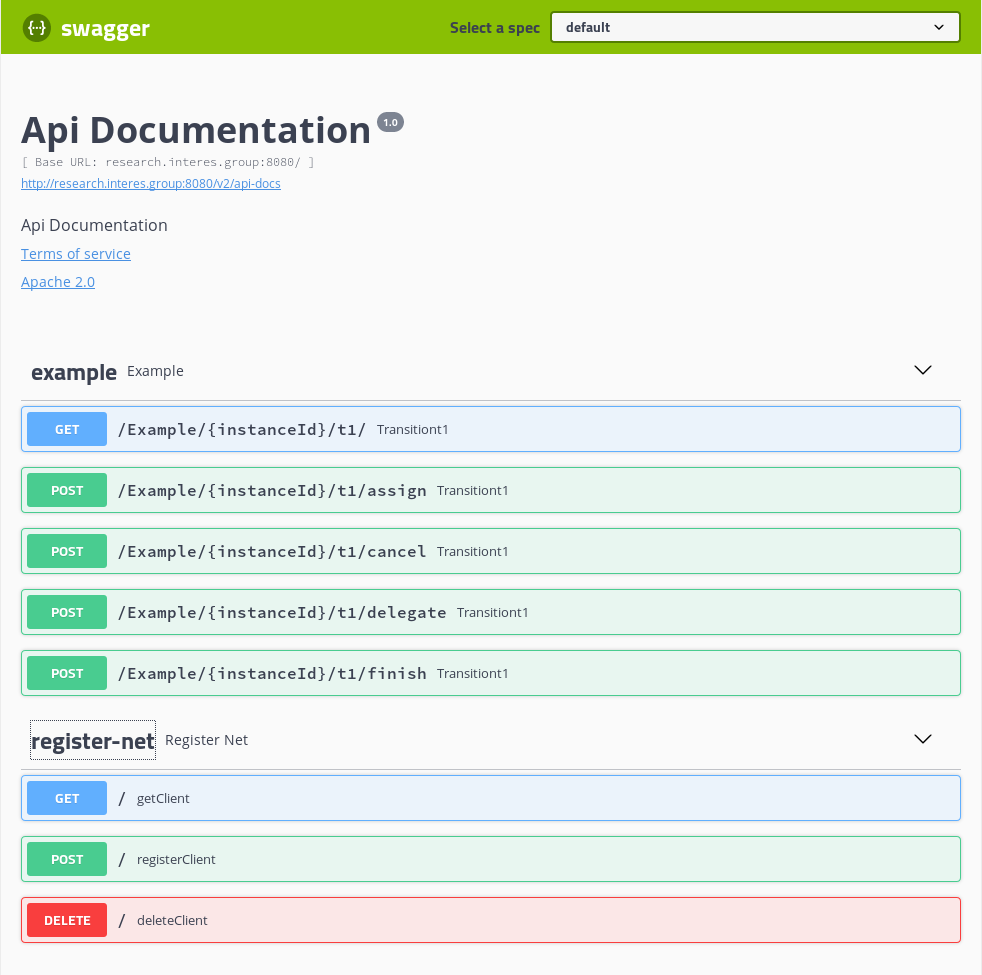
\includegraphics[width=16cm]{img/swagger_ui.png}
	\caption{Ukážka vizualizácie dokumentácie Swagger UI}
	\label{swagger_ui}
\end{figure}

V Swagger UI dokumentácií sa dajú otvoriť jednotlivé koncové body a prezrieť ich detaily. Na obrázku \ref{swagger_ui_endpoint} vidíme príklad detailov koncového bodu finish pre prechod t1. V detailoch vidíme roly, ktoré daný koncový bod môžu použiť, dátové polia, ich typ a či sú povinné. Vidíme tam a aj pole instanceID, ktoré nie je pole z tela dopytu, ale parameter URL.

\begin{figure}[!htbp]
	\centering
	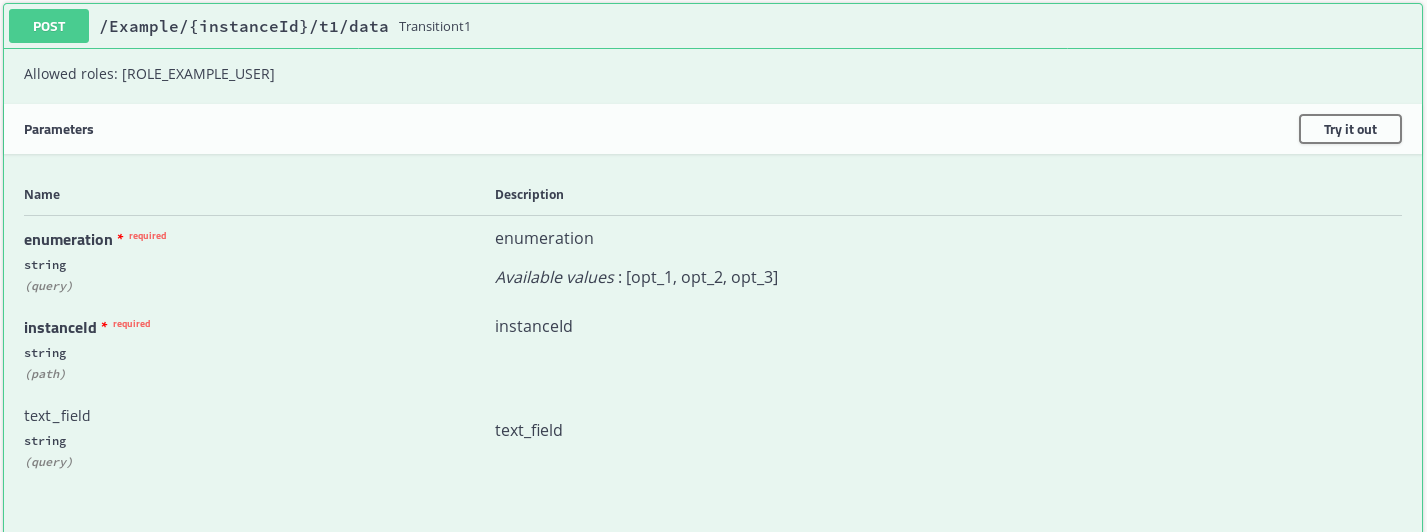
\includegraphics[width=16cm]{img/swagger_ui_endpoint.png}
	\caption{Ukážka vizualizácie dokumentácie kokrétneho koncového bodu}
	\label{swagger_ui_endpoint}
\end{figure}



\subsection{Auth Service}  \label{section_auth}

Na implementáciu autorizačného servera, ktorý dokáže spolupracovať so zvyškom nášho systému sme použili balíček Spring Cloud Security \cite{cloud_security}. Tento balíček podobne ako Spring Boot Security poskytuje základnú funkcionalitu umožňujúcu sa prihlásiť pomocou mena, hesla, alebo aj \acrshort{oauth} a uskladnenie profilov používateľov.

Na rozdiel od základného balíčka Spring Boot Security poskytuje Spring Cloud Security funkcionalitu ktorá umožňuje v centralizovať autentifikáciu do jedného kontajnera. Ostatné kontajnery, ktoré obsahujú koncové body, ktoré chceme zabezpečiť sa označujú ako resource servery.

Resource server, nedrží informácie o používateľoch, ak však príde dopyt na funkciu, ktorá si vyžaduje autorizáciu, vie tento server získať profil používateľa od autorizačného servera. Ak nie je tento používateľ autorizovaný na vykonanie dopytu vracia resource server chybu 403.

Na spustenie autorizačného servera stačí importovať balíky  Spring Cloud Security a Spring Cloud OAuth, napísať základnú konfiguráciu a autorizačný server sa dá spustiť.

Na integráciu so zvyškom nášho systému sme importovali tieto balíky aj do ostatných servisov a v prípade, kedy si funkcionalita vyžiadala autorizáciu  pridali sme potrebné anotácie. Aby sme dosiahli granulárnu kontrolu nad prístupom k funkcionalite, ku každej funkcií sme špecifikovali aké roly k nim majú prístup pomocou príslušnej anotácie.

Pre jednoduchosť implementácie sme na ukladanie profilov používateľov a tokenov využili in memory store. To znamená, že sa pri každom reštarte auth servisu tieto informácie zmažú. Keďže však používame architektúru mikroservisov, a servisy sú od seba do veľkej miery nezávislé, nie je potrebné reštartovať všetky servisy pri zmene jedného. Pri vývoji teda fakt, že používatelia boli uložený vo volatilnej pamäti nebol priveľkou prekážkou. Pre nasadenie systému do produkcie však bude nutné pridať do auth servisu perzistentné úložisko používateľov.

%TODO expand auth service
%TODO auth by classes, by functions

\subsection{Service Discovery}
Service discovery je služba ktorá sleduje stav ostatných služieb a vie zabezpečiť koordináciu komunikácie medzi jednotlivými kontajnermi v cloudovom riešení. V našom systéme implementujeme service discovery ako Spring Boot kontajner s balíčkom Netflix Eureka \cite{eureka}. Nastavenie tohto balička si vyžaduje len importovať závislosť, použiť anot @EnableEurekaServer a nastaviť port servera, v našom prípade je to štandardný port 7777 a hostname Eurka servra.

Na to aby sa ostatné kontajnery zahlásili do service discovery sme importovali v nich balíček Netflix Eureka Client, použili anotáciu @EnableDiscoveryClient a nastavili port, na ktorom sa nachádza discovery servis. Na to aby sme vedeli rozlíšiť typ servisu, ktorý sa pripája na service discovery je ešte potrebné zadať do konfigurácie meno servisu.

Na ukážke kódu \ref{alg:eureka_config} vidíme príklad konfigurácie eureka servra a klienta.

\begin{lstlisting}[float, caption={Konfigurácia Eureka servra a klienta},label={alg:eureka_config},language=yaml]
# Eureka server
server:
  port: 7777
  eureka:
	instance:
	  hostname: localhost
			

# Discovery client	
spring:
  application:
	name: generator-service
eureka:
  client:
	serviceUrl:
	  defaultZone: "http://localhost:7777/eureka"
\end{lstlisting}

Po správnej inicializácií servera a klientov je na porte 7777 dostupná stránka s grafickým rozhraním. Na obrázku \ref{eureka_gui} vidíme screenshoot tejto obrazovky v našom testovacom prostredí. na obrázku vidíme základné informácie o serveri a tabuľku so zaregistrovanými kontajnermi nášho rozhrania. Vidíme, že na porte 8088 beží auth servis, na porte 8080 beží gateway, na porte 8081 beží generátor a na portoch 8082-8085 bežia štyri inštancie relay servisu.

\begin{figure}[!htbp]
	\centering
	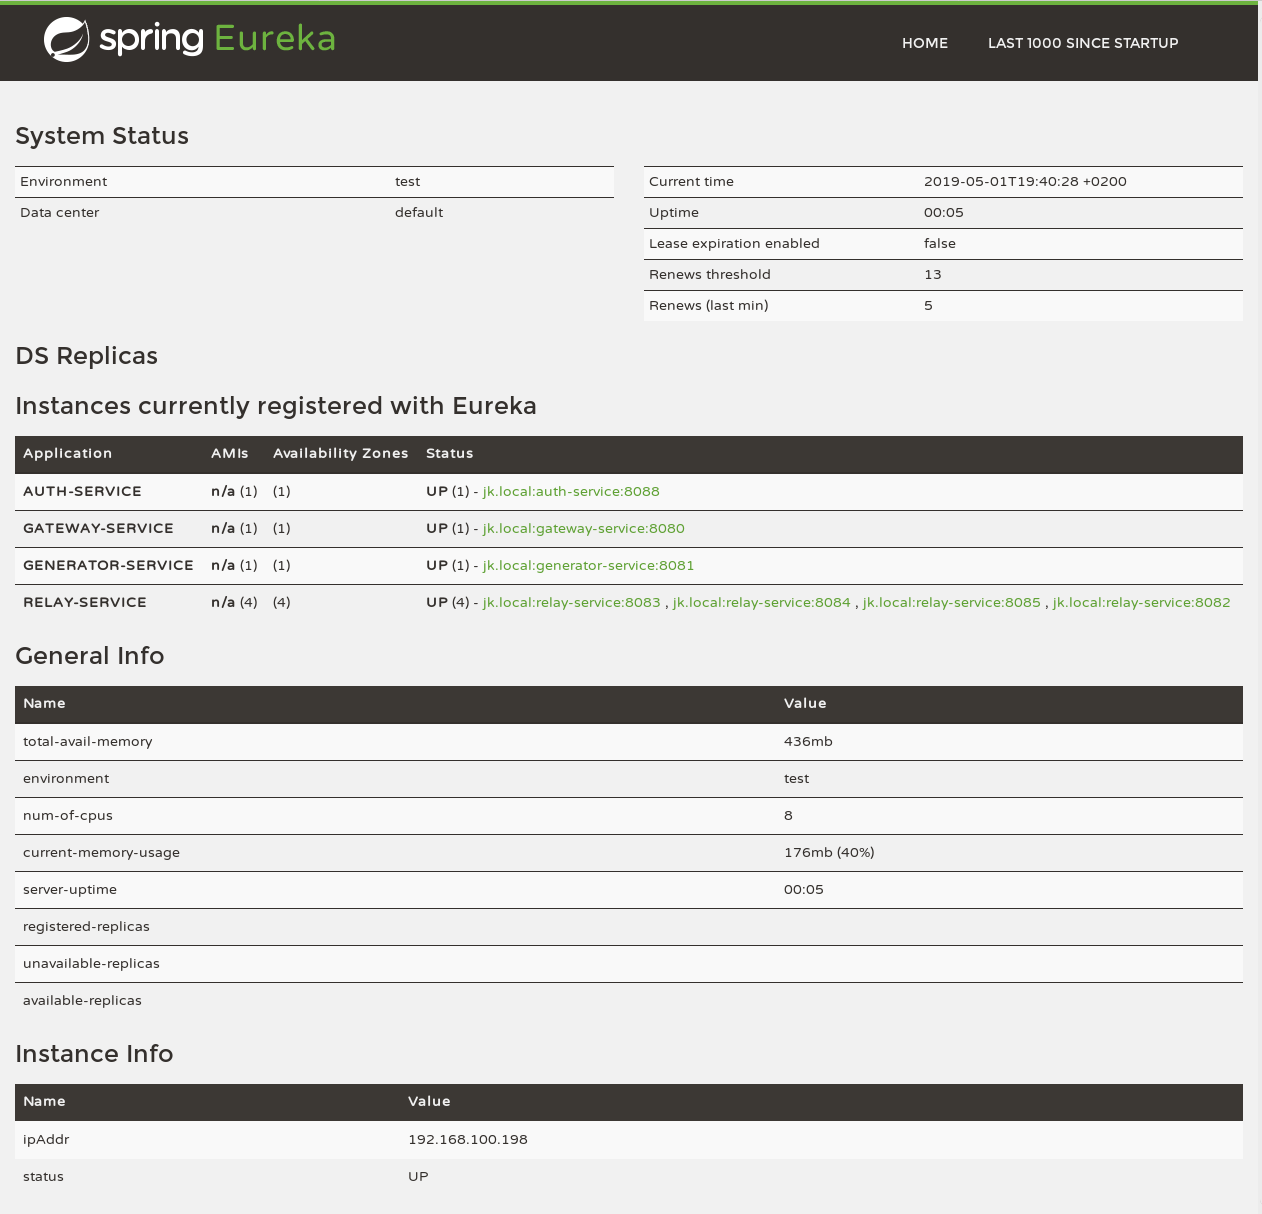
\includegraphics[width=16cm]{img/eureka_gui.png}
	\caption{Užívateľské rozhranie Spring Eureka}
	\label{eureka_gui}
\end{figure}

\subsection{Gateway Service}
Gateway service je rovnako ako ostatné servisy implementovaný ako Spring Boot aplikácia s pridaným balíkom Spring Cloud Gateway \cite{cloud_gateway}, ktorý zabezpečuje funkcionalitu routingu a load balancera.
Na spustenie základnej funkcionality routingu v tomto prípade netreba použiť žiadnu anotáciu, stačí len zadefinovať trasy a k nim prislúchajúce filtre. Na ukážke kódu \ref{alg:gateway_config} vidíme konfiguráciu nášho gateway servisu. Na začiatku je definovaný port na ktorom počúva server, tento port je jediný port, ktorý bude prístupný vonkajšiemu svetu.

\begin{lstlisting}[float, caption={Konfigurácia Gateway servisu},label={alg:gateway_config},language=yaml]
server:
  port: 8080
eureka:
  client:
    serviceUrl:
      defaultZone: http://localhost:7777/eureka/
spring:
  application:
    name: gateway-service
  cloud:
    gateway:
      discovery:
        locator:
          enabled: true
          lower-case-service-id: true
      routes:
        - id: register_route
          uri: "http://localhost:8081/"
          predicates:
            - "Path=/"
        - id: auth_route
          uri: "http://localhost:8088/oauth/"
          predicates:
            - "Path=/oauth/**"
        - id: get_user_route
          uri: "http://localhost:8088/user"
          predicates:
            - "Path=/user"
        - id: endoint_route
          uri: "lb://RELAY-SERVICE/"
          predicates:
            - "Path=/**"
\end{lstlisting}

Prvá \acrshort{url} ktorú máme v konfigurácií zadefinovanú je "/". Táto \acrshort{url} obsahuje funkcie obsluhu nášho rozhrania táto URL je smerovaná na generator service na porte 8081.
Nasledujúce dve trasy smerujú na Auth servis na porte 8088. Prvá obsluhuje dopyty na autentifikáciu cez \acrshort{oauth}, druhá smeruje dopyt na získanie informácií o aktuálnom používateľovi.

Posledná trasa smeruje všetky ostatné dopyty na relay servis. Ako môžeme vidieť URI cieľovej služby nie je s protokolom HTTP a portom na ktorom je služba a ale s protokolom lb a menom služby. Takáto notácia nám umožňuje využiť load balancer balíka Spring Cloud Gateway. Na to aby sme mohli využívať tento protokol musíme ešte nakonfigurovať spojenie so službou service discovery. Ak povolíme možnosť discovery locator, náš gateway servis si vypýta od service discovery informácie o lokácií služieb v našom cloudovom riešení a následne sme schopní adresovať ich pomocou mena, namiesto URI, a môžeme využívať možnosti load balancera. Load balancer sa dá nastaviť aj aby so statickým zoznamom URI jednotlivých inštancii služieb, riešenie cez service discovery locator sa však ukázalo ako praktickejšie, keďže vie dynamicky reagovať na počet spustených inštancií.

Na operáciu gateway servisu nepotrebujeme žiadnu ďalšiu konfiguráciu. Všetky dopyty sú správne smerované servisom, pre ktoré sú určené.

\subsection{Platforma}
V nasledujúcej časti si priblížime aké prostredie sme využívali na vývoj a testovanie systému, ďalej si popíšeme kroky, ktoré sú potrebné na spustenie našej aplikácie

Platforma na ktorú sme nasadzovali náš systém je virtuálny server poskytnutý Fakultou Elektrotechniky a Informatiky na Slovenskej Technickej Univerzite v Bratislave s operačným systémom Ubuntu 18.04.2 LTS Bionic Beaver. Server má k dispozícií 10GB operačnej pamäte, 4GB swap, a 8 jadier procesora.

Pred tým ako sa pokúsime spustiť systém treba sa uistiť, že server, na ktorý plánujeme systém nasadiť bude mať aspoň 8GB voľnej operačnej pamäte a aspoň 2 procesorové jadrá.

Na nasadenie našej aplikácie potrebujeme vykonať nasledovné kroky:
\begin{enumerate}
    \item Uistíme sa, že na serveri je nainštalovaný nástroj Git a Java 8.
	\item Pomocou gitu stiahneme repozitár \cite{dp_repo} s aktuálnou verziou nášho systému.
    \item Skompilujeme a spustíme programu pomocou skriptu "run.sh" ktorý sa nachádza v priečinku repozitára. Tento skript stiahne Gradle 5.4.1, A postupne nainštaluje a spustí všetky kontajnery nášho systému.
	Proces kompilácie a spúšťania kontajnerov je výpočtovo náročný a na serveroch so štyrmi a menej jadrami môže trvať viac ako 3 minúty. Pri prvom spustení si bude inštalačný skript sťahovať závislosti, preto tento proces môže trvať ešte dlhšie.
    \item Povolíme prístup na port 8080 z internetu. 8080 je prednastavený port, na ktorom počúva naša aplikácia. Ak port 8080 nie je vyhovujúci dá sa nastaviť v súbore /gateway/src/resources/application.yml zmenením hodnoty server.port
    \item Na porte 7777 je prezentovane grafické rozhranie service discovery, tento port z bezpečnostných dôvodov neodporúčame povoliť cez firewall, namiesto toho na monitorovanie stavu systému odporúčame použiť ssh tunel pre tento port.
\end{enumerate}



\subsection{Bezpečnosť}
Bezpečnosť je jednou zo základných faktorov ktoré zvážiť pri implementácií akéhokoľvek softvéru. V tejto časti si priblížime ako sme sprístupňovali k bezpečnosti pri návrhu našej aplikácie.  Na obrázku \ref{threat_analysis} vidíme diagram zobrazujúci architektúru nášho systému rozdeleného na rôzne bezpečnostné domény. Ďalej na diagrame môžeme vidieť ako prúdia dáta v našom systéme.  Keď posudzujeme bezpečnosť systému musíme ju posúdiť ako sú bezpečné jednotlivé časti systému, ako napríklad databázy, servery, a zároveň ako je zabezpečená a komunikácia medzi jednotlivými časťami aplikácie, hlavne keď komunikácia prechádza cez hranice bezpečnostnej domény.  

\begin{figure}[!htbp]
	\centering
	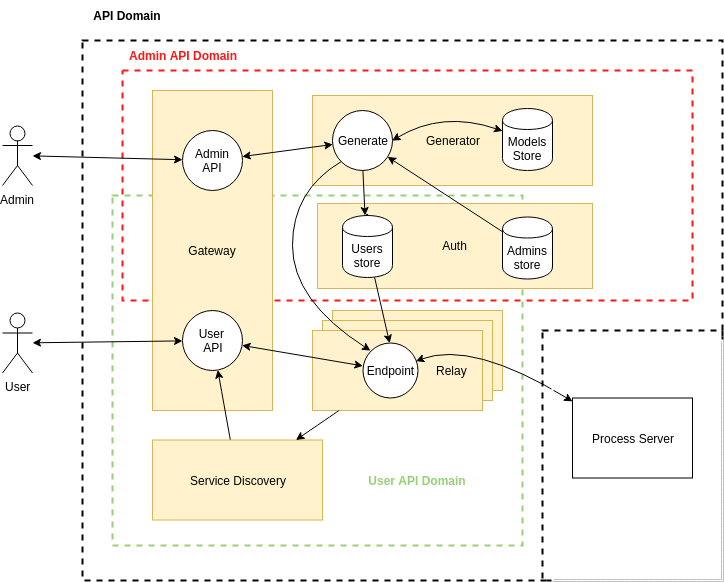
\includegraphics[width=12cm]{img/threat_analysis.png}
	\caption{Diagram Architektúry s bezpečnostnými doménami}
	\label{threat_analysis}
\end{figure}

Komunikácia z internetu do \acrshort{api} domény je chránená tak, že cez firewall serveru je povolený jediný port na prístup do \acrshort{api} domény prístup na tento port je vždy autentifikovaný pomocou protokolu \acrshort{oauth}. V produkčnom prostredí navrhujeme zabezpečiť túto komunikáciu pomocou protokolu HTTPS, aby sa predišlo potenciálnemu úniku dát, prístupových údajov alebo man in the middle útoku. 

Bezpečnosť pri sťahovaní repozitára z Git archívu je zabezpečená pomocou protokolu SSH, ak by sme chceli zvýšiť bezpečnosť mohli by sme si vytvoriť vlastný Git server v rámci našej domény, čo však prináša potrebu tento server udržiavať.

Komunikáciu z \acrshort{api} na procesný server nevieme v tomto bode navrhnúť keďže nevieme v akej doméne sa bude v produkčnom prostredí procesný server nachádzať. Ak by sa však nachádzal mimo domény \acrshort{api} museli by sme komunikáciu zabezpečiť pomocou HTTPS, alebo s pridanou ochranou pomocou VPN alebo SSH tunelu.

Komunikácia v rámci našej domény prebieha pomocou interných protokolov cloudového riešenia v našom prípade HTTP.  Pri testovaní a vývoji je naše riešenie nasadené celé v rámci jedného virtuálneho servera preto nepovažujeme za potrebné zabezpečovať túto komunikáciu. Ak by však produkčné prostredie bolo nasadené na viacerých virtuálnych alebo fyzických serveroch odporúčame použitie šifrovania spojenia. Na zabezpečenie šifrovanej komunikácie môžeme použiť šifrovanie jednotlivých spojení pomocou SSH, alebo využitie hotového riešenia na komunikáciu v rámci cloudových kontajnerov.

V rámci našej aplikácie sa nachádzajú dve domény, administrátorská a používateľská. V administrátorskej doméne sa nachádza služba generator. Ak by útočník získal kontrolu nad touto službou bol by schopný obmedziť funkčnosť nášho používateľského klientského rozhrania, zamedziť prístup používateľom k aplikačnému rozhraniu alebo naopak povoliť neoprávnenej osobe prístup k rozhraniu. Ak by útočník vypol  tento servis, neobmedzila by  sa schopnosť \acrshort{api} odpovedať na používateľské dopyty obmedzila  by sa len schopnosť meniť rozhranie. Náš systém bude implementovaný tak, aby administrátor mal prístup k rozhraniu z internetu. Prístup ku generator servisu je len pomocou dopredu definovaných autentifikovaných HTTP volaní. Pre zvýšenie bezpečnosti v produkčnom prostredí odporúčame povolenie prístupu na generator servis len z vnútra našej domény, napr pomocou VPN/SSH.

V používateľskej doméne sa nachádza relay servis. Ak by nad týmto servisom získal útočník kontrolu, mohol by neoprávnene spúšťať prechody a získavať dáta z prechodov na procesnom serveri. Keďže relay servis je vždy spustený vo viacerých inštanciách na obmedzenie funkčnosti prostredia by musel útočník vypnúť všetky inštancie relay servisu. Ak by útočník Všetky volania na relay servis sú autentifikované pomocou \acrshort{oauth}.  Aby sme ochránili procesný server proti SQL injection útokom navrhujeme v produkčnom prostredí presne špecifikovať formát vstupu pre jednotlivé typy polí a  implementovať čistenie vstupov pomocou štandartných nástrojov.

Gateway servis sám o sebe nespracováva žiadne používateľské dpyty iba ich smeruje ďalej do systému. Toto obmedzuje výber útokov možný na tento servis. Voči gateway servisu môže útočník použiť útok DDOS, V produkčnom prostredí sa takémuto útoku môžeme brániť použitím rate limitera. Ak by útočík získal kontrolu nad týmto servisom mohol by aplikačné rozhranie znefunkčniť alebo mu nížiť priepustnosť.

Service discovery komunikuje iba na pomocou svojho protokolu s ostatnými kontajermi v siei, takze opäť je výber útokov obmedzený. Keďe tneto servis používame sledovanie počtu a stavu inštancií relay servisu na účely load balalncingu, mohol by útočník reportovať iný počet alebo inú lokáciu inštancií relay servisu a tým obmedziť priepustnosť alebo znefunkčniť rozhranie.

Auth servis zasahuje do oboch našich bezpečnostných domén. Prihlasovacie údaje a roly sú však oddelené rôznym menným priestorom, to nám zaručuje, že pri registrácií nových rolí sa používatelia nemôžu dostať k prostriedkom, ktoré patria do administrátorskej domény. Samotnú
autentifikáciu v našej aplikácií rieši auth servis pomocou štandardnej implementácie \acrshort{oauth}. Tento protokol zabezpečuje dostačujúci stupeň bezpečnosti pri autentifikácií. Útok pomocou napadnutia registrácie používateľov sme už spomenuli vyššie pri generator servise. Ak by útočník získal kontrolu nad auth servisom vedel by obmedziť prístup oprávneným používateľom, alebo neoprávnene získať prístup ku koncovým bodom relay servisu.

V produkčnom prostredí taktiež odporúčame nasadiť riešenie na centralizované skladovanie logov zo všetkých servisov.

%todo toto do zhodnotenia?
Architektúram mikroservisov prináša do serverových systémov vysoký výkon a škálovateľnosť no tým, že sa skladá z viacerých oddelených servisov ktoré musia medzi sebou komunikovať, prináša zo sebou aj riziko napadnutia tejto komunikácie. Ak však vieme zaručiť bezpečnosť tejto komunikácie uzavretím systému do bezpečnej domény, alebo šifrovaním jednotlivých komunikačných kanálov, z bezpečnostného hľadiska je táto architektúra vyhovujúca na  implementáciu bezpečných a vysoko škálovateľných systémov


\section{Testovanie}
V tejto kapitole si priblížime proces testovania ktorý sme využívali pri vývoji systému a systém automatizovaného testovania, ktorý sme implementovali na systéme.

\subsection{Manuálne testy}

Na manuálne testovanie počas vývoja sme používali softvér Insomnia REST Client\cite{insomnia}. V tomto programe sme vytvorili rôzne volania na náš systém a kontrolovali sme ich výstup.

\subsubsection{Auth service}
Pri autorizačnom serveri sme testovali, či základným systémovým používateľom bude správne pridelený autorizačný token a či tento token je platný. Na obrázku \ref{insomnia_oauth} vidíme príklad takéhoto dopytu. Na príklade vidíme, že po vyplnení správnych údajov do karty OAuth 2 v programe Insomnia môžeme odoslať dopyt na zabezpečený koncový bod v našej aplikácií a dopyt vráti správnu odpoveď.
\begin{figure}[!htbp]
	\centering
	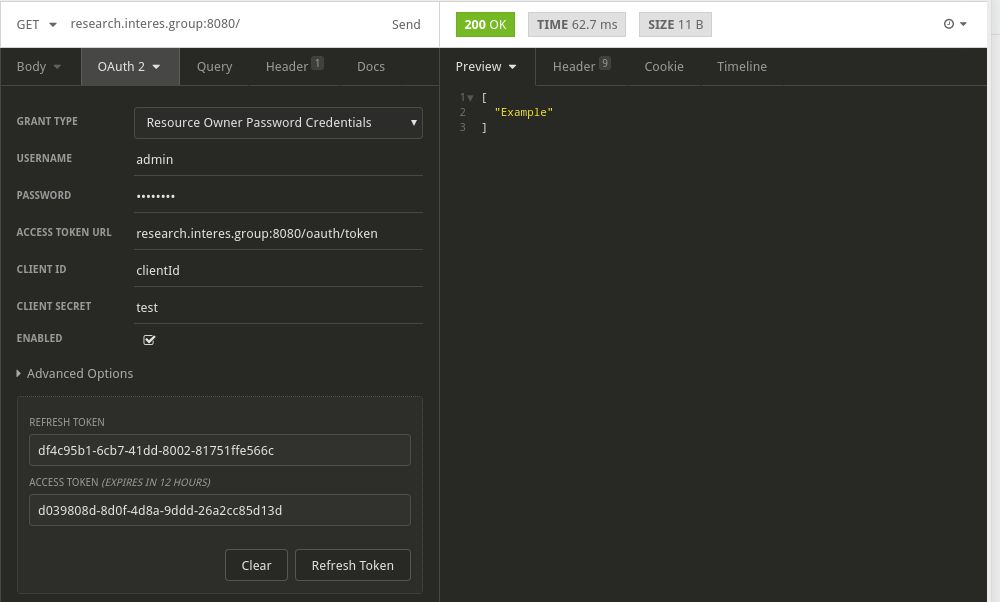
\includegraphics[width=16cm]{img/insomnia_oauth.png}
	\caption{Ukážka testu auth servisu}
	\label{insomnia_oauth}
\end{figure}

\subsubsection{Gateway service}
Pri gateway service sme testovali správne nastavenie smerovania, a či server naozaj smeruje dotazy na správny server. Ďalej sme testovali funkcionalitu load balancera. Tú sme testovali tak, že sme spustili viaceré inštancie relay servisu, s miernymi zmenami v kóde a load balancer naše dopyty smeroval striedavo na rôzne inštancie relay servisu.

\subsubsection{Generator service}
Pri generator service sme testovali či sa vygeneroval spustiteľný kód. V prípade, že kód ktorý sa vygeneroval nebol syntakticky správny vrátil koncový bod generátora chybovú odpoveď. Jedna z chýb ktoré sme pri takomto testovaní objavili je chyba knižnice kotlinpoet, kedy sa pri generovaní zalomí dlhší text bez ošetrenia úvodzoviek a teda sa vygeneruje nevalidný kód.

Ak sa korektne vygeneroval kód a spustila sa nová inštancia relay servisu testovali sme, či vygenerovaný kód validácie funguje korektne.

Ďalej sme pri tejto službe testovali, či sa pri regenerácií relay servisu prejavila zmena v dokumentácií korektne, a či sa správne zaregistrovali používatelia v auth servise.

\subsubsection{Relay service}
Pri tomto servise sme testovali funkčnosť validačných funkcií. Testovali sme, či neprítomnosť povinného dátového poľa vráti správnu chybovú hlášku, a či pri poliach s predpísaným formátom vstupu vráti servis chybu ak formát vstupu nie je korektný a či ak je formát správny prebehne funkcia korektne a vráti pozitívny výsledok. Na obrázku \ref{insomnia_200} vidíme príklad korektného dotazu a na obrázku \ref{insomnia_400} vidíme príklad dopytu, ktorý nemá správny formát dát v poli s enumeráciou.

\begin{figure}[!htbp]
	\centering
	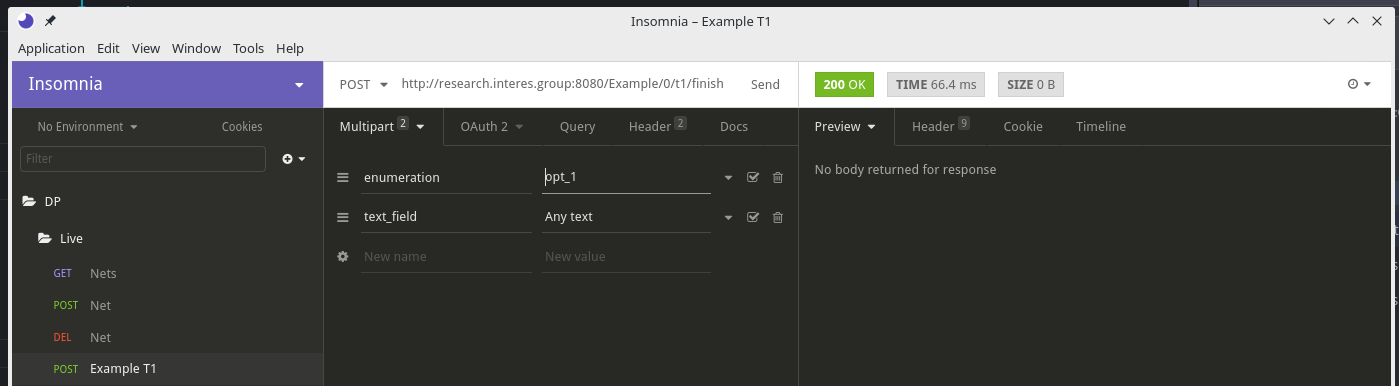
\includegraphics[width=16cm]{img/insomnia_200.png}
    \caption{Ukážka vizualizácie dokumentácie konkrétneho koncového bodu}
	\label{insomnia_200}
\end{figure}

\begin{figure}[!htbp]
	\centering
	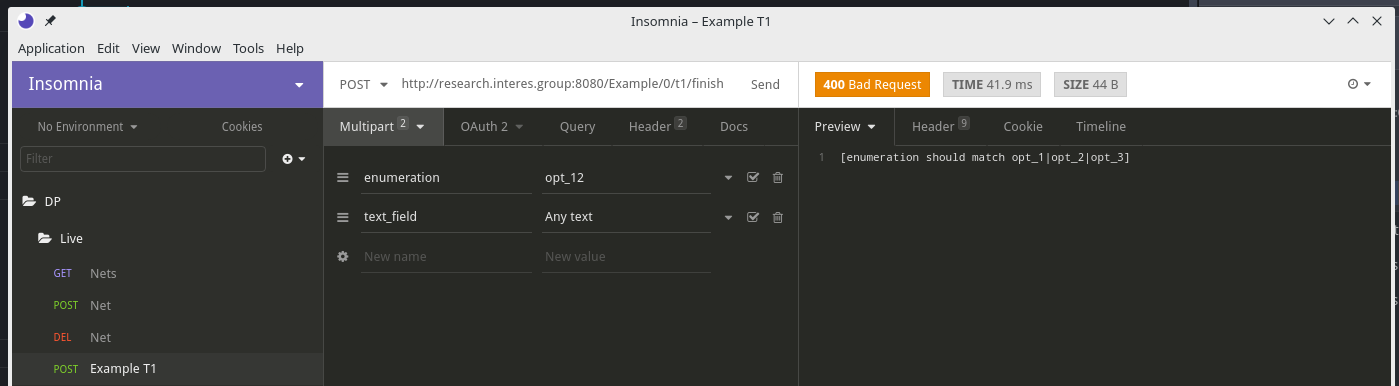
\includegraphics[width=16cm]{img/insomnia_400.png}
    \caption{Ukážka vizualizácie dokumentácie konkrétneho koncového bodu}
	\label{insomnia_400}
\end{figure}

\subsection{Automatizované testy}

%TODO auto test relay service
